\subsection{环上的整元素}

定理 1. 设 A 是（交换）环，R 是 A 上的代数（未必交换），x 是 R 的元素。下列性质等价：

(E \(_{I}\) ) x 是多项式环 A{[}X{]} 中一个首一多项式的根。

\((\mathbf{E}_{\mathrm{II}})\) 子代数 \(\mathbf{A}[x]\) （\(\mathbf{R}\) 的）是有限生成 A-模。

\((E_{\mathrm{III}})\) 存在环 A{[}x{]} 上的一个忠实模，它是有限生成 A-模。

先证 \((\mathbf{E}_{\mathbf{I}})\) 蕴涵 \((\mathbf{E}_{\mathbf{II}})\) 。设

\[
\mathrm{X} ^ {n} + a _ {1} \mathrm{X} ^ {n - 1} + \dots + a _ {n}
\]

是 A{[}X{]} 中以 x 为根的一个首一多项式；对每个整数 \(q \geqslant 0\) ，设 \(M_{q}\) 是 R 的由 1、\(x, \ldots, x^{n+q}\) 生成的子 A-模。那么

\[
x ^ {n + q} = - a _ {1} x ^ {n + q - 1} - \dots - a _ {n} x ^ {q} \in \mathrm{M} _ {q - 1}
\]

对所有 \(q \geqslant 1\) 成立，于是由对 \(q\) 的归纳法得

\[
\mathbf {M} _ {q} = \mathbf {M} _ {q - 1} = \dots = \mathbf {M} _ {0}.
\]

由此得出 A{[}x{]} 等于 \(M_{0}\) ，从而是有限生成 A-模。

由于交换环 A{[}x{]} 是自身上的忠实模，\((\mathbf{E}_{\mathrm{II}})\) 蕴涵 \((\mathbf{E}_{\mathrm{III}})\) 。

最后，\((\mathbf{E}_{\mathrm{III}})\) 蕴涵 \((\mathbf{E}_{\mathrm{I}})\) 这一事实将由下面更精确的引理得出：

引理 1. 设 A 是环，R 是 A 上的代数（未必交换），x 是 R 的元素。设 M 是 A{[}x{]} 上的忠实模且是有限生成 A-模。若 q 是 A 的理想使得 xM ⊂ qM，则 x 是一个系数属于 A 的首一多项式的根，该多项式中除首项系数外的所有系数都属于 q。

设 \((u_{i})_{1\leqslant i\leqslant n}\) 是 M 的元素的有限族，使得 \(\mathbf{M} = \sum_{i = 1}^{n}\mathbf{A}u_{i}\) 。对所有 \(i\) ，由假设存在 q 的元素的有限族 \((q_{ij})_{1\leqslant j\leqslant n}\) 使得

\[
x u _ {i} = \sum_ {j = 1} ^ {n} q _ {i j} u _ {j} \quad \text { for } \quad 1 \leqslant i \leqslant n.
\]

因此（《代数》，第 III 章，§ 8），若 \(d\) 是矩阵 \((q_{ij} - \delta_{ij}x)\) （元素在 A{[}x{]} 中）的行列式（ \(\delta_{ij}\) 表示 Kronecker 指标），则 \(du_i = 0\) 对所有 \(i\) 成立，从而 \(d\mathbf{M} = 0\) ；由于 M 假设是忠实 A{[}x{]}-模，必有 \(d = 0\) 。这表示 \(x\) 是多项式 \(\det(q_{ij} - \delta_{ij}\mathbf{X})\) （在 A{[}X{]} 中的）的根，该多项式相差一个符号便是一个首一多项式，其除首项系数外的系数都属于 q。

定义 1. 设 A 是环，R 是 A-代数（未必交换）。称元素 \(x \in \mathbb{R}\) 为 \(A\) 上的整元素，如果它满足定理 1 的等价性质 \((\mathrm{E}_{\mathrm{I}}), (\mathrm{E}_{\mathrm{II}}), (\mathrm{E}_{\mathrm{III}})\) 。

形如 \(\mathrm{P}(x)=0\) 的关系（其中 P 是 A{[}X{]} 中的首一多项式）也称为系数在 A 中的整依赖关系方程。

\textbf{例}\par

\begin{enumerate}
\def\labelenumi{(\arabic{enumi})}
\tightlist
\item
  设 K 是（交换）域，R 是 K-代数；说元素 \(x \in R\) 在 K 上是整的，等价于说 x 是环 K{[}X{]} 中某个非常数多项式的根；把 R 是 K 的扩域时引入的术语（《代数》，第 V 章，§3，第 3 节）加以推广，R 中在 K 上为整的元素 \(x \in R\) 也称为 R 在 K 上的代数元素。
\end{enumerate}

* (2) \(\mathbf{Q}(i)\) 中在 \(\mathbf{Z}\) 上为整的元素是形如 \(a + ib\) 的元素，其中 \(a \in \mathbf{Z}\) 且 \(b \in \mathbf{Z}\) （``Gauss 整数''）；\(\mathbf{Q}(\sqrt{5})\) 中在 \(\mathbf{Z}\) 上为整的元素是形如 \((a + b\sqrt{5})/2\) 的元素，其中 \(a\) 与 \(b\) 属于 \(\mathbf{Z}\) 且同为偶数或同为奇数（这两个例子见习题 1）。*

\begin{enumerate}
\def\labelenumi{(\arabic{enumi})}
\setcounter{enumi}{2}
\tightlist
\item
  在 \(\mathbf{Z}\) 上为整的复数也称为代数整数。
\end{enumerate}

\textbf{注}\par

\begin{enumerate}
\def\labelenumi{(\arabic{enumi})}
\item
  设 A' 是 R 的子环（含于 R 的中心），即在定义 R 上 A-代数结构的环同态 A → R 下 A 的像。显然，说 R 的一个元素在 A 上是整的，等价于说它在 A' 上是整的。
\item
  设 \(R'\) 是 R 的子 A-代数；\(R'\) 中在 A 上为整的元素恰是 R 中在 A 上为整且属于 \(R'\) 的元素；这常使我们在不致混淆时无需指明 A 上的整元素属于哪个代数。
\end{enumerate}

命题 1. 设 A 是环，R 是 A 上的代数（未必交换），x 是 R 的元素。要使 x 在 A 上是整的，必须且只需 A{[}x{]} 含于 R 的一个子代数 R' 中，且该子代数是有限生成 A-模。

由性质 \((\mathrm{E}_{\mathrm{II}})\) ，条件显然必要；它也充分，由 \((\mathrm{E}_{\mathrm{III}})\) ，因为 \(R'\) 是忠实 A{[}x{]}-模（因为它含 R 的单位元素）。

推论. 设 A 是 Noether 环，R 是 A-代数（未必交换），x 是 R 的元素。要使 x 在 A 上是整的，必须且只需存在 R 的一个有限生成子模包含 A{[}x{]}。

由 \((\mathrm{E}_{\mathrm{II}})\) 条件必要；它充分，因为若 A{[}x{]} 是某个有限生成 A-模的子 A-模，则它本身是有限生成 A-模（《代数》，第 VIII 章，§2，第 3 节，命题 7）。

\pandocbounded{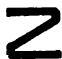
\includegraphics[keepaspectratio]{images/part002_1e1abfe7.jpg}}

A 是 Noether 环这一假设不能从陈述中略去（习题 2）。

定义 2. 设 A 是环。若 A-代数 R（未必交换）的每个元素都在 A 上是整的，则称 R 在 A 上是整的。若 R 是有限生成 A-模，则称 R 在 A 上是有限的。

由命题 1，每个有限 A-代数都是整的；若 R 是交换的且是有限 A-代数，则 R 显然是有限生成 A-代数；反之不真。

例（4）若 M 是有限生成 A-模，则 M 的自同态代数 \(\operatorname{End}_{\mathbf{A}}(\mathbf{M})\) 由 \((\mathrm{E}_{\mathrm{III}})\) 在 A 上是整的；特别地，对每个整数 n，矩阵代数 \(\mathbf{M}_{n}(\mathbf{A}) = \operatorname{End}_{\mathbf{A}}(\mathbf{A}^{n})\) 在 A 上是整的（甚至是有限的）。

命题 2. 设 A、A' 是两个环，R 是 A-代数，R' 是 A'-代数（未必交换），\(f\colon\mathbf{A}\to\mathbf{A}'\) 与 \(g\colon\mathbf{R}\to\mathbf{R}'\) 是两个环同态，使得图表

\pandocbounded{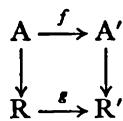
\includegraphics[keepaspectratio]{images/part002_4af46373.jpg}}

交换。若元素 \(x \in R\) 在 A 上是整的，则 \(g(x)\) 在 \(A'\) 上是整的。若 \(x^{n} + a_{1}x^{n-1} + \cdots + a_{n} = 0\) ，其中 \(a_{i} \in A\) （ \(1 \leqslant i \leqslant n\) ），我们推出

\[
(g (x)) ^ {n} + f \left(a _ {1}\right) (g (x)) ^ {n - 1} + \dots + f \left(a _ {n}\right) = 0.
\]

推论 1. 设 A 是环，B 是（交换）A-代数，C 是（未必交换）B-代数。那么在 A 上为整的每个元素 \(x \in \mathbf{C}\) 在 B 上也是整的。

推论 2. 设 K 是域，L 是 K 的扩域，x、\(x'\) 是 L 的两个在 K 上共轭的元素（《代数》，第 V 章，§ 6，第 2 节）。若 A 是 K 的子环且 x 在 A 上是整的，则 \(x'\) 也在 A 上是整的。

存在一个 K-同构 \(f\) ，它把 \(\mathbf{K}(x)\) 映到 \(\mathbf{K}(x')\) 上，使得 \(f(x) = x'\) ，且 \(\mathbf{A}\) 的元素在 \(f\) 下不变。

推论 3. 设 A 是环，B 是（交换）A-代数，C 是（未必交换）B-代数。若 C 在 A 上是整的，则 C 在 B 上是整的。

命题 3. 设 \((\mathbf{R}_i)_{1\leqslant i\leqslant n}\) 是（未必交换）的

A-代数的有限族，设 \(\mathbf{R} = \prod_{i=1}^{n} \mathbf{R}_i\) 是它们的乘积。要使元素 \(x = (x_i)_{1 \leq i \leq n}\) （\(\mathbf{R}\) 的）在 \(\mathbf{A}\) 上是整的，必须且只需每个 \(x_i\) 都在 \(\mathbf{A}\) 上是整的。要使 \(\mathbf{R}\) 在 \(\mathbf{A}\) 上是整的，必须且只需每个 \(\mathbf{R}_i\) 都在 \(\mathbf{A}\) 上是整的。

显然只需证明第一个断言。条件必要由命题 2 得出。反之，若每个 \(x_{i}\) 都在 \(A\) 上是整的，则子代数 \(A[x_{i}]\) （\(R_{i}\) 的）是有限生成 \(A\) -模，因而 R 的子代数 \(\prod_{i=1}^{n} \mathrm{A}[x_i]\) 也是；由于 \(\mathrm{A}[x]\) 含于这个子代数，由命题 1，\(x\) 在 A 上是整的。

命题 4. 设 A 是环，R 是 A-代数（未必交换），\((x_{i})_{1\leq i\leq n}\) 是 R 的两两可交换元素的有限族。若对所有 \(i, x_{i}\) 都在 \(A[x_{1},\cdots,x_{i-1}]\) 上是整的（特别地，若所有 \(x_{i}\) 都在 A 上是整的），则 R 的子代数 \(A[x_{1},\ldots,x_{n}]\) 是有限生成 A-模。

我们对 \(n\) 作归纳论证，命题就是 \((\mathbf{E}_{\mathrm{II}})\) （当 \(n = 1\) 时）。归纳假设蕴涵 \(B = A[x_{1}, \cdots, x_{n-1}]\) 是有限生成 A-模；由于 \(x_{n}\) 在 B 上是整的，\(B[x_{n}] = A[x_{1}, \cdots, x_{n}]\) 是有限生成 B-模，从而也是有限生成 A-模（《代数》，第 II 章，§ 1，第 13 节，命题 25）。

推论 1. 设 A 是环，R 是（交换）A-代数。R 中在 A 上为整的元素组成的集是 R 的一个子代数。

事实上，若 x, y 是 R 的两个在 A 上为整的元素，则由命题 4，A{[}x, y{]} 是有限生成 A-模；由于它含 \(x + y\) 与 xy，推论由命题 1 得出。

\pandocbounded{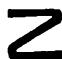
\includegraphics[keepaspectratio]{images/part002_90735efb.jpg}}

在非交换代数中，两个 A 上整元素的和与积未必在 A 上是整的（习题 4）。

推论 2. 设 A 是环，R 是 A-代数（未必交换），E 是 R 中两两可交换且在 A 上为整的元素组成的集。则 R 的由 E 生成的子 A-代数 B 在 A 上是整的。

B 的每个元素都属于 B 的一个由 E 的有限子集生成的子 A-代数。

注（3）由命题 4 推出，每个在 A 上为整的交换 A-代数都是 A 上有限子代数的一个右有向族的并。

命题 5. 设 A 是环，A' 与 R 是两个（交换）A-代数。若 R 在 A 上是整的，则 \(R \otimes_{A} A'\) 在 A' 上是整的。

考虑任一元素 \(x' = \sum_{i=1}^{n} x_i \otimes a_i'\) （\(\mathbf{R} \otimes_{\mathbf{A}} \mathbf{A}'\) 的），其中 \(x_i\) 属于 \(\mathbf{R}\) ，\(a_i'\) 属于 \(\mathbf{A}'\) ；由于 \(x_i \otimes a_i' = (x_i \otimes 1)a_i'\) 且诸 \(x_i \otimes 1\) 在 \(\mathbf{A}'\) 上是整的（命题 2），\(x\) 亦然。

推论. 设 R 是环，A、B、C 是 R 的子环，使得 \(A \subset B\) 。若 B 在 A 上是整的，则 C{[}B{]} 在 C{[}A{]} 上是整的。

\(B \otimes_{A} C[A]\) 由命题 5 在 \(C[A]\) 上是整的，因而典范像 \(C[B]\) （\(B \otimes_{A} C[A]\) 在 \(R\) 中的，R 视为 A-代数）由命题 2 也是。

命题 6. 设 A 是环，B 是（交换）A-代数，C 是（未必交换）B-代数。若 B 在 A 上是整的且 C 在 B 上是整的，则 C 在 A 上是整的。

只需验证每个 \(x \in C\) 在 A 上是整的。由假设存在一个系数在 B 中且以 x 为根的首一多项式 \(X^{n} + b_{1}X^{n-1} + \cdots + b_{n}\) ；于是 x 在 \(B' = A[b_{1}, \ldots, b_{n}]\) 上是整的，从而 \(B'[x]\) 是有限生成 \(B'\) -模。但由于 B 在 A 上是整的，\(B'\) 是有限生成 A-模（命题 4）；我们断定 \(\mathbf{B}'[x]\) 也是有限生成 A-模（《代数》，第 II 章，§1，第 13 节，命题 25），因而 \(x\) 在 \(\mathbf{A}\) 上是整的。

推论. 设 A 是环，R、R' 是两个在 A 上为整的（交换）A-代数。则 \(R \otimes_{A} R'\) 在 A 上是整的。

\(R \otimes_{A} R'\) 在 \(R'\) 上是整的（命题 5），因而结论由命题 6 得出。

